\section{Optimizations}

The program as described in section \vref{sec:implementation} is
unoptimized and written for readability and simplicity. This section
deals with potential and realized optimizations. Optimizing one aspect
of performance can often hurt another aspect. See section
\vref{sec:specs} for the specifications of the test computer. Programs
were translated with \texttt{gcc} version 4.4.5 and the following flags:
\texttt{-O3 -march=i686}.

\subsection{Finding out where}
\label{sec:finding_out_where}
The first step in optimizing should be finding out where. To this
purpose we have set up a few experiments to decide the memory usage
and runtimes of the programs. In all the following experiments, the
first program, \texttt{main}, in our pipe is called with a regular
expression matching capturing all: \textsf{(.*)} and about 114KB of
text generated by \url{lipsum.com} to be matched. 

%% In all experiments the first program,
%% \texttt{main}, was called with a regular expression matching text
%% between two bold tags:
%% \begin{center}
%% \textsf{.*\textless B\textgreater ((?:(?:(?:\textless (?:/B\textless \textbar /\textless \textbar \textless )*(?:/B[\^{}\textless \textgreater ]\textbar /[\^{}\textless B]\textbar [\^{}\textless /]))\textbar [\^{}\textless ])*)[\textless /B]*)\textless /B\textgreater .*}
%% \end{center}
%% and a string consisting of about 71K bytes of text generated by
%% \url{www.lipsum.com} with bold tags at either end as arguments. The
%% rest of the programs was called with appropriate output as input. The
%% output was saved in files and piped in where needed. 

\subsubsection{Memory usage}
In table \vref{tab:memory_usage} we have the peak memory usage
charted. These numbers were collected with \texttt{valgrind} using the
parameters \texttt{--tool=massif --stacks=yes}. These parameters mean
we collect information on stack and heap usage. We can see from the
table that all programs except \texttt{trace} use a negligible amount
of memory. The Perl script in section \vref{sec:memoryusage.pl} was
used for collecting the data in this paragraph.

\ctable[
  caption = Peak memory usage,
  label = tab:memory_usage
]
{lr|lr}
{}
{\FL
 Program & Size (KB) & Program & Size (KB) \ML
\texttt{main} & 3.43 & \texttt{groupings\_all} & 3.43 \\
\texttt{trace} & 1500.16 & \texttt{serialize} & 3.43 \\
\texttt{ismatch} & 3.43 \LL
}

\subsubsection{Output sizes}
The sizes of the output from the previous experiment on memory usage
is plotted in figure \vref{tab:output_size}. We can see that there is
a big size difference between input to \texttt{main} and output; the
output is 9 times bigger than the input. The same goes for the output
of \texttt{groupings\_all}, this is because there is nothing to be
removed by this filter with this particular regular expression. The
output of \texttt{trace} is 3 times bigger than the original string of
text.

\ctable[
  caption = Sizes of output,
  label = tab:output_size
]
{lr|lr}
{}
{\FL
 Program & Size (KB) & Program & Size (KB) \ML
\texttt{main} & 1022.5 & \texttt{groupings\_all} & 1022.5 \\
\texttt{trace} & 340.8 & \texttt{serialize} & 113.6 \\
\texttt{ismatch} & 0 \LL
}


\subsubsection{Runtimes}
We made a small experiment to decide the runtimes of each program. We
used the Perl script in section \vref{sec:runtimes.pl} to measure
runtimes. We used the regular expression \textsf{(.*)} and a logfile
of suitable size as inputs. In table \vref{tab:runtimes} the runtimes
for the different programs is seen. \lstinline{trace} takes more than
5 hours to complete.

\ctable[
  caption = Runtimes,
  label = tab:runtimes
]
{lr|lr}
{}
{\FL
 Program & Runtime (s) & Program & Runtime (s) \ML
\texttt{main} & 1.010 & \texttt{groupings\_all} & 2.168 \\
\texttt{trace} & 18762.863 & \texttt{serialize} & 0.443 \\
\texttt{ismatch} & 0.773 \LL
}


%% \begin{figure}
%%   \centering
%%   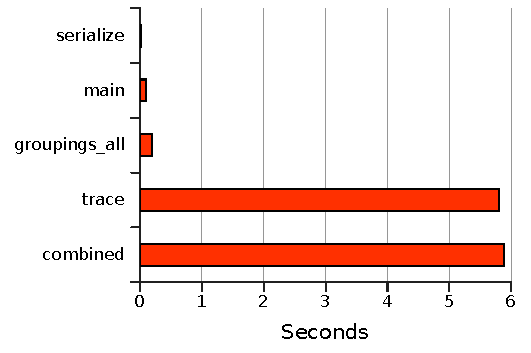
\includegraphics{optimizations/runtimes.pdf}
%%   \caption{Runtimes for the programs}
%%   \label{fig:runtimes}
%% \end{figure}
\subsubsection{Profiling}
We need to analyze the runtime behavior of the programs, to see which
functions takes up the runtime of the programs. This is what a profiler
is for. There are many to chose from. We chose to use \texttt{gprof}
as it can give us an overview of which functions are called and how
much time is spent in each.

The programs was compiled and linked with the \texttt{-pg} option to
enable profiling data to be collected for \texttt{gprof}. We need to
extend the runtimes to get better results from \texttt{gprof}, so
instead of the text from \url{lipsum.com} we used a logfile of
suitable size. The size was chosen to be small enough to fit in
memory, but big enough to produce longer runtimes. In section
\vref{sec:profiling.pl} we have the perl script used for the
profiling.

In figures \ref{fig:main_unoptimized},
\ref{fig:groupings_all_unoptimized}, \ref{fig:trace_unoptimized} and
\ref{fig:serialize_unoptimized} we have the output from
\texttt{gprof} flat profile column marked \texttt{\% time}. This
column describes the percentage of the total running time used by this
function. Only functions taking up more than 5\% of the total runtime
is included, the rest is bunched together in the other column.

\paragraph{\texttt{main}}
\begin{figure}
  \centering
  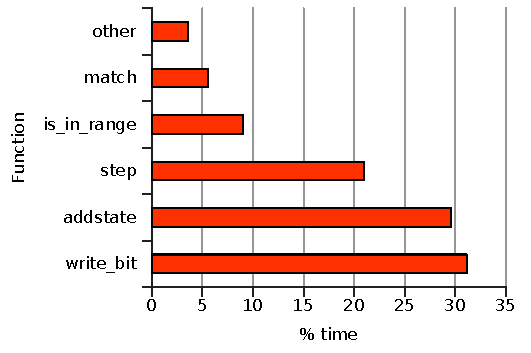
\includegraphics[]{optimizations/main_unoptimized.pdf}
  \caption{Output of \texttt{gprof} running \texttt{main}}
  \label{fig:main_unoptimized}
\end{figure}
In figure \vref{fig:main_unoptimized} we have the values for running
\texttt{main}. Functions \lstinline{add_state}, \lstinline{step},
\lstinline{is_in_range} and \lstinline{match} is all called in the
process of simulating the NFA, this takes up about 65\% of the total
runtime. The rest is taken up by IO: Function
\lstinline{write_bit}. For this example, the process of creating the
NFA is near instantaneous. We can also see the penalty for choosing a
simple solution to the character class problem, the function for
deciding membership \lstinline{is_in_range} takes up about 9\% of the
total runtime.

\paragraph{\texttt{groupings\_all}}
\begin{figure}
  \centering
  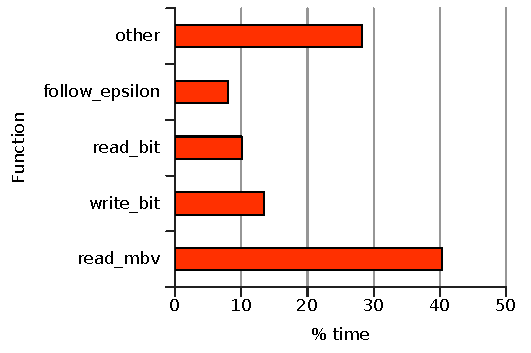
\includegraphics[]{optimizations/groupings_all_unoptimized.pdf}
  \caption{Output of \texttt{gprof} running \texttt{groupings\_all}}
  \label{fig:groupings_all_unoptimized}
\end{figure}
In figure \vref{fig:groupings_all_unoptimized} we have the values for
running \texttt{groupings\_all}. The main loop function,
\lstinline{read_mbv} takes up about 40\% of the total runtime. We also
see a large amount of runtime being taken up by functions with a small
amount of runtime each, these are helper functions to the main loop
and functions to do with keeping track of the channels. Again does the
IO functions \lstinline{write_bit} and \lstinline{read_bit} take up a
fair amount of runtime, about 23\%.

\paragraph{\texttt{trace}}
\begin{figure}
  \centering
  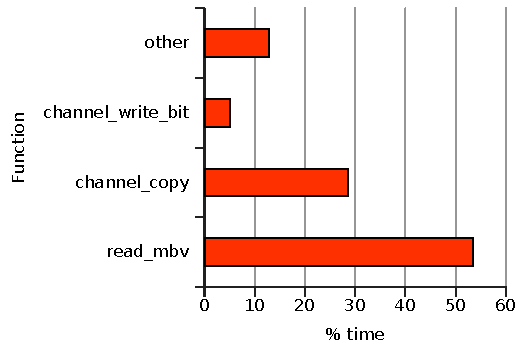
\includegraphics[]{optimizations/trace_unoptimized.pdf}
  \caption{Output of \texttt{gprof} running \texttt{trace}}
  \label{fig:trace_unoptimized}
\end{figure}
In figure \vref{fig:trace_unoptimized} we have the values for running
\texttt{trace}. The main loop function \lstinline{read_mbv} takes up
more than half the total runtime. We spend a lot of time copying,
writing to, appending and freeing channels, about 40\% of the total
runtime. Functions prepended with a \lstinline{channel_} deal with
channel management. Here the IO functions \lstinline{read_bit} and
\lstinline{write_bit} take up a relatively little amount of runtime,
about 5\% in total.

\paragraph{\texttt{serialize}}
\begin{figure}
  \centering
  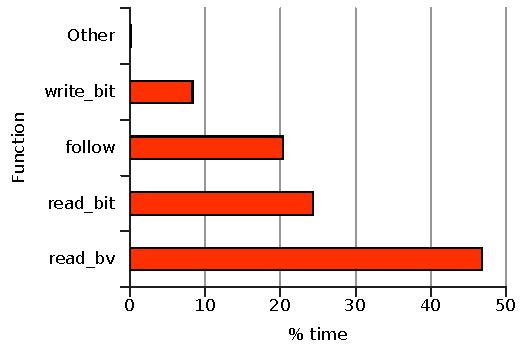
\includegraphics{optimizations/serialize_unoptimized.pdf}
  \caption{Output of \texttt{gprof} running \texttt{serialize}}
  \label{fig:serialize_unoptimized}
\end{figure}
In figure \vref{fig:serialize_unoptimized} we have the values for
running \texttt{serialize}. Again the main loop function takes up a
lot of time, about 47\% of the total runtime. I/O functions
\lstinline{read_bit} and \lstinline{write_bit} takes up about a third
of the total runtime.

\subsection{Applying the knowledge gained}

In the previous section we identified a few troublespots, these are
listed here. 
\begin{description}
\item[IO] From the output of \texttt{gprof} we can see that a lot of
  our runtime, in most programs, is used in the two I/O functions
  \lstinline{read_bit} and \lstinline{write_bit}.
\item[\texttt{trace}] \lstinline{trace} takes to long to complete, a
  good place to start would be to look for a way around all the
  channel management.
\item[Main loops] A lot of the runtime is spend in main loops. This is
  not necessarily a good place to start optimizing, this could just as
  well be because we were not good at spreading out the workload in
  smaller functions.
\end{description}


\subsubsection{$\upvarepsilon$-lookahead}

Each $\upvarepsilon$-transition is marked with a look-ahead
symbol. The $\upvarepsilon$-transition can then only be taken if the
look-ahead symbol matches the next character in the input string. This
optimization will have double effect, it will both reduce the number
of states in the active set when simulating the NFA and it will reduce
the mixed bit-values output at the cost of extra memory for and time
spend constructing the NFA.

This optimization has not been implemented.

\subsubsection{Improved protocol encoding}
The protocol used for transmitting data is text-based, using a binary
protocol would make the content more terse, but also nigh impossible
to read for a human. 

To transmit one operator in the text based protocol we always use 8
bits. Since we only have 8 different operators, this can be done using
less bits. A widely used and effective technique for lossless
compression of data is Huffman codes \cite{Cormen}. To encode our data
efficiently with Huffman codes we need to analyze our data; we need to
know the frequency with which the operators appear. In table
\vref{tab:huffman_freq} we have some frequencies of the operators
using different regular expressions on a text file generated by
\url{www.lipsum.org} of size 114KB. We have a simple and a somewhat
complex example. Since this is a table of operator frequencies, we
have left out the escaped characters, this means the numbers will not
sum to 100. What is missing is the escaped characters, these have the
same frequency as the escape operator.

\ctable[
  caption = Frequencies of operators in a mixed bit-value string,
  label = tab:huffman_freq
]{l|rr}{
  \tnote[a]{\textsf{.*}}
  \tnote[b]{\textsf{(?:(?:(?:[a-zA-Z]+ ?)+[,.;:] ?)*..)*}}
}{\FL
Operator & Match all\tmark[a] & Match words\tmark[b]\ML
\texttt{0} & 11\% & 13\% \NN
\texttt{1} & 11\% & 13\% \NN
\texttt{:} & 22\% & 27\% \NN
\texttt{\textbar} & 11\% & 2\% \NN
\texttt{=} & 11\% & 13\% \NN
\texttt{\textbackslash} & 11\% & 8\% \NN
\texttt{b} & 11\% & 13\% \NN
\texttt{t} & 0\% & 0\% \LL
}

In figures \vref{fig:huffman1} and \vref{fig:huffman2} we have the
corresponding Huffman trees, they yield the encoding in table
\vref{tab:huffman_codes}. We observe that as the regular expression
gets more complicated, we use \texttt{\textbar} and
\texttt{\textbackslash} less and \texttt{0}, \texttt{1}, \texttt{:},
\texttt{=} and \texttt{b} more. This is also reflected in the Huffman
encoding. Since most regular expression will be more complex than
\textsf{.*}, we choose the encoding in the match words column. This
gives us a compression ratio of 0.39, for the match words case
and a compression ratio of 0.44 for the match all case. 

\ctable[
  caption = Huffman encoding,
  label = tab:huffman_codes
]{l|rr}{
  \tnote[a]{\textsf{.*}}
  \tnote[b]{\textsf{(?:(?:(?:[a-zA-Z]+ ?)+[,.;:] ?)*..)*}}
}{\FL
Operator & Match all\tmark[a] & Match words\tmark[b]\ML
\texttt{0}              & 1110 & 010   \NN
\texttt{1}              & 010  & 110   \NN
\texttt{:}              & 00   & 10    \NN
\texttt{\textbar}       & 011  & 01110 \NN
\texttt{=}              & 100  & 111   \NN
\texttt{\textbackslash} & 101  & 0110  \NN
\texttt{b}              & 110  & 00    \NN
\texttt{t}              & 1111 & 01111 \LL
}

We can not make assumptions beforehand as to the frequencies of the
escaped characters. Their frequency depends highly on the text being
matched. If the escaped characters all have the same frequency, then
the Huffman method can achieve no compression. Instead we can look to
the character class that generated the escaped character. By rewriting
the character class with the \textsf{\textbar} operator and creating
the corresponding partial NFA as a balanced tree and use this tree as
we would a Huffman tree, we can compress the escaped characters. How
efficient this method is depends on how many characters is matched by
the character class. For example if we match all characters, then no
compression would be obtained, if on the other hand we had a small
character class like \textsf{[a-d]} we could encode characters matched
by this class using only 2 bits. 

We did not implement this optimization.

\subsubsection{Buffering input and output}

%% \begin{figure}
%%   \centering
%%   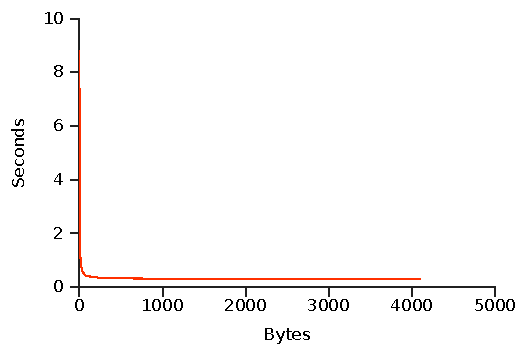
\includegraphics[]{optimizations/buffersize.pdf}
%%   \caption{Combined runtimes with different buffersize for input and output}
%%   \label{fig:buffersize}
%% \end{figure}
\ctable[
  caption = Runtimes for different buffersizes,
  label = tab:buffersize
]{rr|rr}{
}{\FL
Buffer size (B) & Runtime (s) & Buffer size (B) & Runtime (s)\ML
0   &   8.786 & 128 &	0.391\NN
2   &	4.507 & 256 &	0.338\NN
4   &	2.559 & 512 &	0.320\NN 
8   &	1.354 & 1024&	0.313\NN
16  &	0.886 & 2048&	0.314\NN
32  &	0.618 & 4096&	0.310\NN
64  &	0.437 & 8196&   0.324\LL
}

The two functions called when doing I/O is \lstinline{fputc} and
\lstinline{fgetc}. These are included with the \texttt{stdio.h} header
file. Reading up on those two reveal that they are buffered and
thread-safe. There is even a function for manipulating the buffering
method: \lstinline{setvbuf}. We did a bit of experimenting with
\lstinline{setvbuf}, the results are shown in figure
\vref{tab:buffersize}. The runtimes in the graph is the combined
runtime of all programs, i.e. we measured the runtime for all programs
combined with pipes:
\begin{verbatim}
echo lipsum | ./main regex | ./groupings_all regex  |  \
./trace | ./serialize regex'
\end{verbatim}
\texttt{regex} and \texttt{lipsum} are the same as used in section
\vref{sec:finding_out_where}. We can see that not much is gained from
a buffer size exceeding 1024 bytes.

\paragraph{Thread-safety}
We also looked into thread safety. There are non-thread-safe variants of
\lstinline{fputc} and \lstinline{fgetc}, \lstinline{fputc_unlocked}
and \lstinline{fgetc_unlocked} respectively. Note that the man-pages
does state that these thread-unsafe functions probably should not be
used. The results from an experiment similar to the previous, only
using the non-thread-safe functions for IO, are in table
\vref{tab:buffersize_unlocked}. The non-thread-safe functions are on
average 0.16 seconds faster. 

\ctable[
  caption = Runtimes for different buffersizes using non-thread-safe functions,
  label = tab:buffersize_unlocked
]{rr|rr}{
}{\FL
Buffer size (B) & Runtime (s) & Buffer size (B) & Runtime (s)\ML
0	&8.597 & 128	&0.248 \NN
2	&4.355 & 256	&0.204 \NN
4	&2.288 & 512	&0.181 \NN
8	&1.240 & 1024	&0.177 \NN
16	&0.716 & 2048	&0.164 \NN
32	&0.463 & 4096	&0.151 \NN
64	&0.308 & 8192	&0.162 \LL
}


%% Experimenting with the
%% \lstinline{setvbuf} function gave no improvement in runtimes. We can
%% also try looking into the threadsafety. There are thread-unsafe
%% variants of \lstinline{fputc} and \lstinline{fgetc},
%% \lstinline{fputc_unlocked} and \lstinline{fgetc_unlocked}
%% respectively. This gave some results, note that the man-pages does
%% state that these thread-unsafe functions probably should not be
%% used. We can also implement our own buffering mechanism and call
%% functions \lstinline{fputs} and \lstinline{fgets} instead. These two
%% functions read/write a whole line instead of a single character. This
%% also gave some results. 


\subsubsection{Channel management in \lstinline{trace}}

The problem with \lstinline{trace} is that we do not know which
channel has a match, so we need to keep track of the bit-values on all
of them. If we instead read the mixed bit-values backwards, the first
character we would read on a channel would be the \texttt{t} or
\texttt{b} operator, precluding the problem of knowing which channel
has a match. This does require us to read the whole string of mixed
bit-values and reversing it. Because this filter already is
non-streaming, it will not become a problem reading and storing the
whole string of mixed bit-values.

This optimization is implemented. Running the experiments determining
runtime and memory usage for the improved \texttt{trace} gives us a
runtime of just 1.309 seconds and a memory usage of 1536KB. Comparing
this to the values for the old \lstinline{trace} we see a huge
performance gain in runtime and a slight increase in memory
consumption. This optimization is well worth it.

We would expect no performance gain on this optimization when the
regular expression consists of a string of literals, that is we only
create one channel when simulating the NFA. This is however not a very
useful application of regular expressions, there are faster ways of
comparing two strings.
